\section{Gravity Plume On a Continental Slope}
%\label{www:tutorials}
\label{sec:eg-gravityplume}
\begin{rawhtml}
<!-- CMIREDIR:eg-gravityplume: -->
\end{rawhtml}
\begin{center}
(in directory: {\it verification/tutorial\_plume\_on\_slope/})
\end{center}

\begin{rawhtml}MITGCM_INSERT_FIGURE_BEGIN T-plume-on-slope\end{rawhtml}
\begin{figure}
\begin{center}
\includegraphics[width=\textwidth,height=.3\textheight]{s_examples/plume_on_slope/billows.eps}
\end{center}
\caption{Temperature after 23~hours of cooling. The cold dense water is
mixed with ambient water as it accelerates down the slope and hence
is warmed than the unmixed plume.
}
\label{fig:T-plume-on-slope}
\end{figure}
\begin{rawhtml}MITGCM_INSERT_FIGURE_END\end{rawhtml}

An important test of any ocean model is the ability to represent the
flow of dense fluid down a slope. One example of such a flow is a
non-rotating gravity plume on a continental slope, forced by a limited
area of surface cooling above a continental shelf. Because the flow is
non-rotating, a two dimensional model can be used in the across slope
direction. The experiment is non-hydrostatic and uses open-boundaries
to radiate transients at the deep water end.  (Dense flow down a slope
can also be forced by a dense inflow prescribed on the continental
shelf; this configuration is being implemented by the DOME (Dynamics
of Overflow Mixing and Entrainment) collaboration to compare solutions
in different models). The files for this experiment can be found in
the verification directory under tutorial\_plume\_on\_slope.

The fluid is initially unstratified.  The surface buoyancy loss $B_0$
(dimensions of L$^2$T$^{-3}$) over a cross-shelf distance $R$ causes
vertical convective mixing and modifies the density of the fluid by an
amount
\begin{equation}
\Delta \rho = \frac{B_0 \rho_0 t}{g H}
\end{equation}
where $H$ is the depth of the shelf, $g$ is the acceleration due to
gravity, $t$ is time since onset of cooling and $\rho_0$ is the
reference density. Dense fluid slumps under gravity, with a flow speed
close to the gravity wave speed:
\begin{equation}
U
\sim \sqrt{g' H}
\sim \sqrt{ \frac{g \Delta \rho H}{\rho_0} }
\sim \sqrt{B_0 t}
\end{equation}
A steady state is rapidly established in which the buoyancy flux out of 
the cooling region is balanced by the surface buoyancy loss. 
Then 
\begin{equation}
U \sim (B_0 R)^{1/3} \mbox{  ;  } \Delta \rho \sim \frac{\rho_0}{g H} (B_0 R)^{2/3} 
\end{equation}
The Froude number of the flow on the shelf is close to unity (but in 
practice slightly less than unity, giving subcritical flow). 
When the flow reaches the slope, it accelerates, so that it may become 
supercritical (provided the slope angle $ \alpha $ is steep enough). 
In this case, a hydraulic control is established at 
the shelf break. On the slope, where the Froude number is greater 
than one, and gradient Richardson number 
(defined as $Ri \sim g' h^*/U^2$ where $h^*$ is the thickness of the 
interface between dense and ambient fluid) is reduced 
below 1/4, Kelvin-Helmholtz instability is possible, and leads to 
entrainment of ambient fluid into the plume, modifying the 
density, and hence the acceleration down the slope. 
Kelvin-Helmholtz instability is suppressed at low Reynolds and 
Peclet numbers given by 
\begin{equation}
Re \sim \frac{U h}{ \nu} \sim \frac{(B_0 R)^{1/3} h}{\nu} \mbox{  ;  } Pe = Re Pr
\end{equation}
where $h$ is the depth of the dense fluid on the slope. 
Hence this experiment is carried out in the high Re, Pe regime. 
A further constraint is that the convective heat flux must be much greater 
than the diffusive heat flux (Nusselt number $>> 1$). 
Then 
\begin{equation}
Nu = \frac{U h^* }{\kappa} >> 1
\end{equation}
Finally, since we have assumed that the convective mixing on the shelf
occurs in a much shorter time than the horizontal equilibration, 
this implies $H/R << 1$.  

Hence to summarize the important nondimensional parameters, and 
the limits we are considering:
\begin{equation}
\frac{H}{R} << 1 \mbox{ ; } Re >> 1 \mbox{  ; } Pe >> 1 \mbox{  ; } Nu >> 1
\mbox{  ;  } \mbox{  ; } Ri < 1/4 
\end{equation}
In addition we are assuming that the slope is steep enough to provide 
sufficient acceleration  to the gravity plume, but nonetheless much less 
that $1:1$, since many Kelvin-Helmholtz billows appear on the slope, 
implying horizontal lengthscale of the slope $>>$ the depth of the 
dense fluid. 

\subsection{Configuration}
%\label{www:tutorials}

The topography, spatial grid, forcing and initial conditions are all
specified in binary data files generated using a {\em Matlab} script
called {\tt gendata.m} and detailed in
section~\ref{sec:plume-generating}. Other model parameters are
specified in file {\tt data} and {\tt data.obcs} and detailed in
section~\ref{sec:plume-params}.

\subsection{Binary input data}
%\label{www:tutorials}
\label{sec:plume-generating}

\begin{figure}
\begin{center}
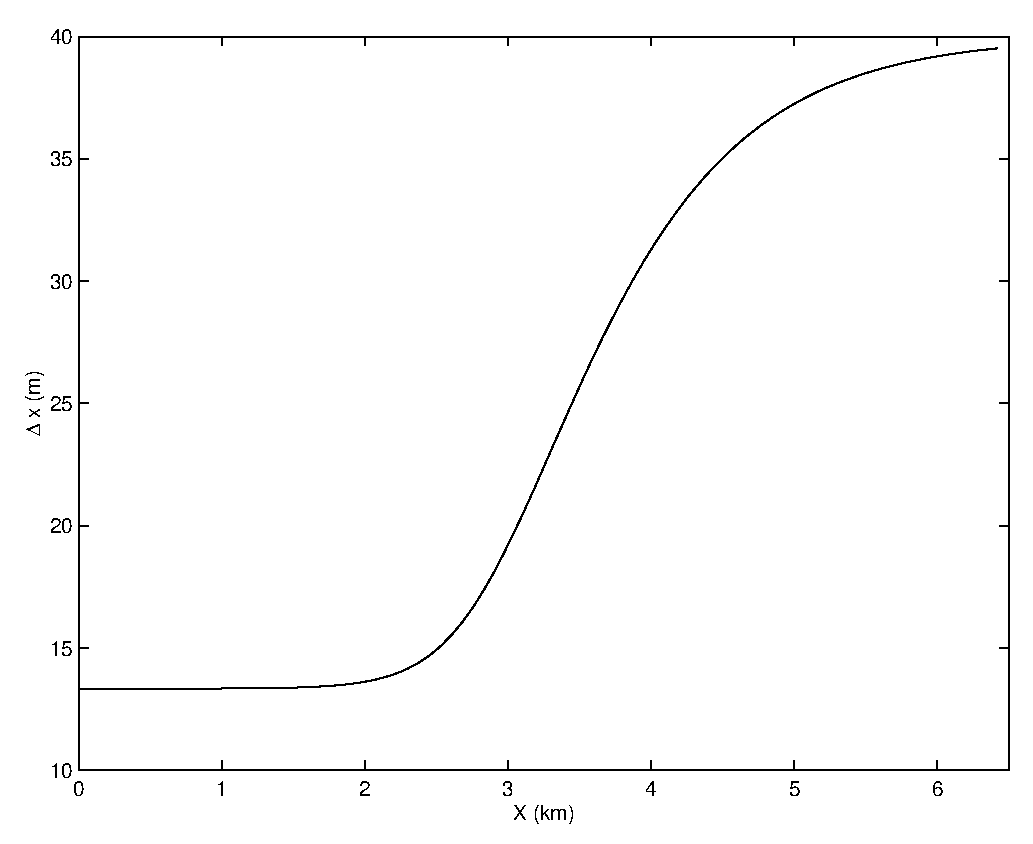
\includegraphics[width=\textwidth,height=.3\textheight]{s_examples/plume_on_slope/dx.eps}
\end{center}
\caption{Horizontal grid spacing, $\Delta x$, in the across-slope
direction for the gravity plume experiment.}
\label{fig:dx-plume-on-slope}
\end{figure}

\begin{figure}
\begin{center}
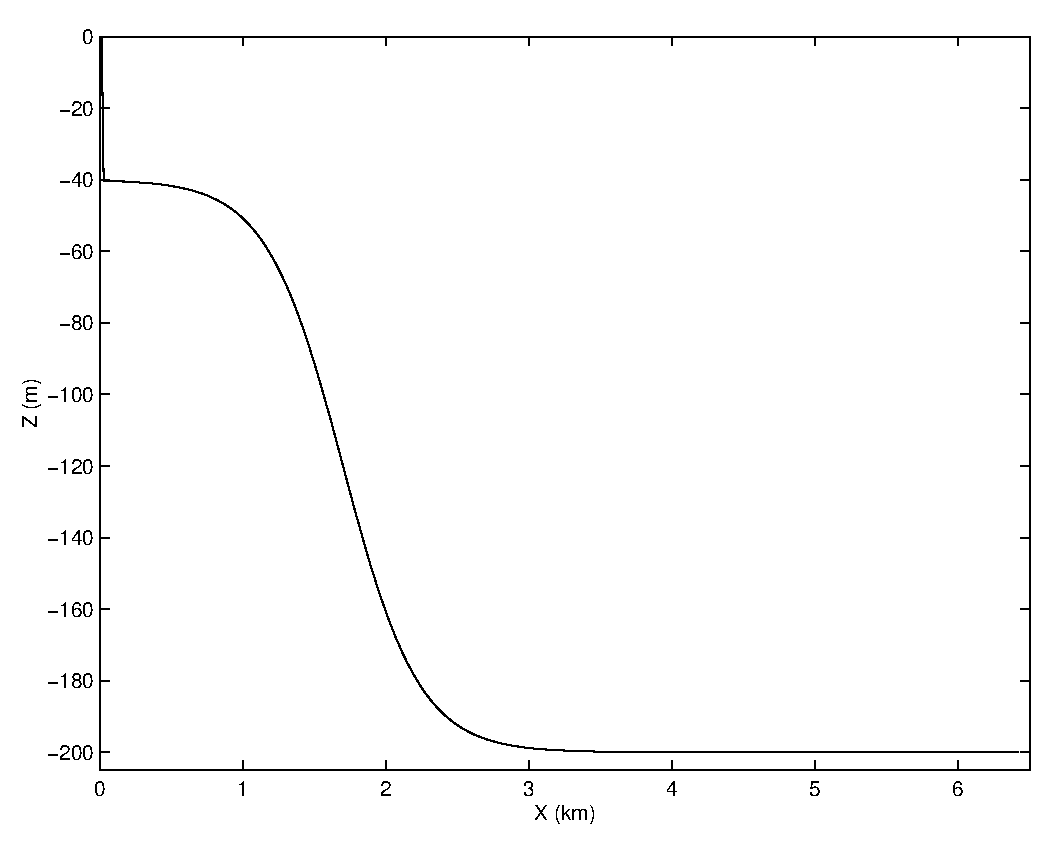
\includegraphics[width=\textwidth,height=.3\textheight]{s_examples/plume_on_slope/Depth.eps}
\end{center}
\caption{Topography, $h(x)$, used for the gravity plume experiment.}
\label{fig:depth-plume-on-slope}
\end{figure}

\begin{figure}
\begin{center}
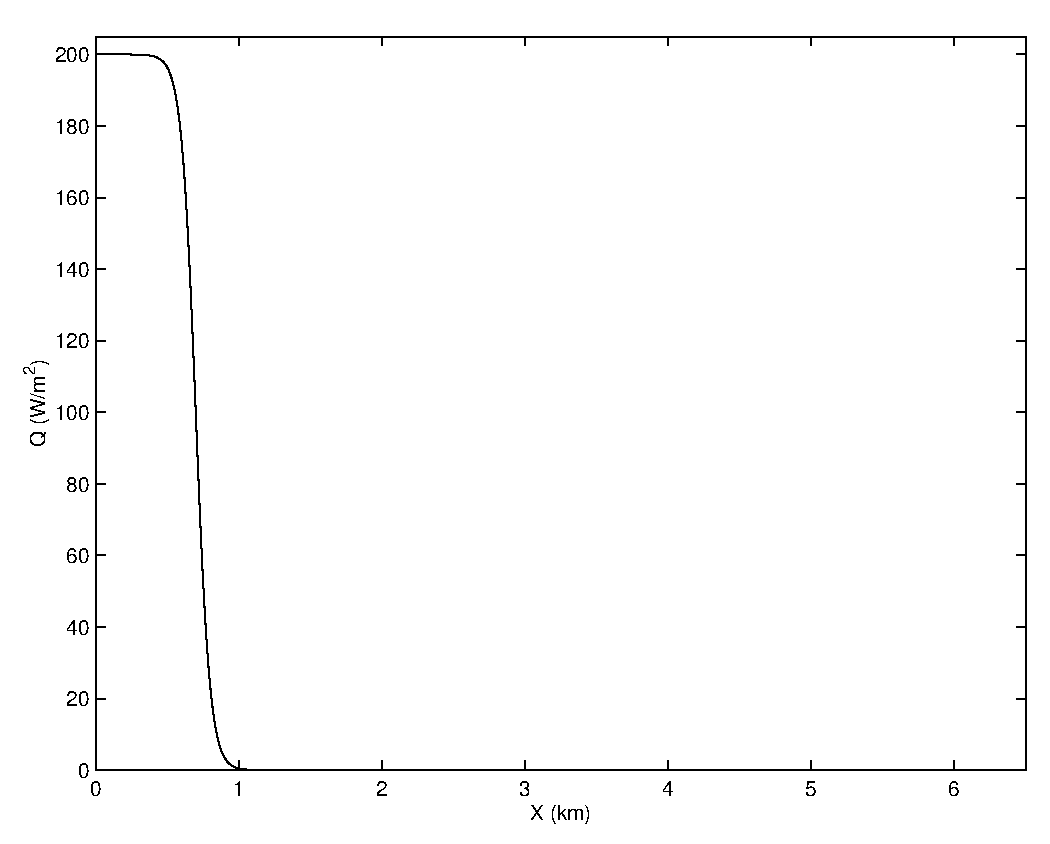
\includegraphics[width=\textwidth,height=.3\textheight]{s_examples/plume_on_slope/Qsurf.eps}
\end{center}
\caption{Upward surface heat flux, $Q(x)$, used as forcing in the
gravity plume experiment.}
\label{fig:Q-plume-on-slope}
\end{figure}

The domain is $200$~m deep and $6.4$~km across. Uniform resolution of
$60\times3^1/_3$~m is used in the vertical and variable resolution of
the form shown in Fig.~\ref{fig:dx-plume-on-slope} with $320$ points
is usedin the horizontal. The formula for $\Delta x$ is:
\begin{displaymath}
\Delta x(i) = \Delta x_1 + ( \Delta x_2 - \Delta x_1 )
( 1 + \tanh{\left(\frac{i-i_s}{w}\right)} ) /2
\end{displaymath}
where
\begin{eqnarray*}
Nx & = & 320 \\
Lx & = & 6400 \;\; \mbox{(m)} \\
\Delta x_1 & = & \frac{2}{3} \frac{Lx}{Nx} \;\; \mbox{(m)} \\
\Delta x_2 & = & \frac{Lx/2}{Nx-Lx/2 \Delta x_1} \;\; \mbox{(m)} \\
i_s & = & Lx/( 2 \Delta x_1 ) \\
w & = & 40 
\end{eqnarray*}
Here, $\Delta x_1$ is the resolution on the shelf, $\Delta x_2$ is the
resolution in deep water and $Nx$ is the number of points in the
horizontal.

The topography, shown in Fig.~\ref{fig:depth-plume-on-slope}, is given
by:
\begin{displaymath}
H(x) = -H_o + (H_o - h_s) ( 1 + \tanh{\left(\frac{x-x_s}{L_s}\right)} ) / 2
\end{displaymath}
where
\begin{eqnarray*}
H_o & = & 200 \;\; \mbox{(m)} \\
h_s & = & 40 \;\; \mbox{(m)} \\
x_s & = & 1500 + Lx/2 \;\; \mbox{(m)} \\
L_s & = & \frac{(H_o - h_s)}{2 s} \;\; \mbox{(m)} \\
s & = & 0.15
\end{eqnarray*}
Here, $s$ is the maximum slope, $H_o$ is the maximum depth, $h_s$ is
the shelf depth, $x_s$ is the lateral position of the shelf-break and
$L_s$ is the length-scale of the slope.

The forcing is through heat loss over the shelf, shown in
Fig.~\ref{fig:Q-plume-on-slope} and takes the form of a fixed flux
with profile:
\begin{displaymath}
Q(x) = Q_o ( 1 + \tanh{\left(\frac{x - x_q}{L_q}\right)} ) / 2
\end{displaymath}
where
\begin{eqnarray*}
Q_o & = & 200 \;\; \mbox{(W m$^{-2}$)} \\
x_q & = & 2500 + Lx/2 \;\; \mbox{(m)} \\
L_q & = & 100 \;\; \mbox{(m)}
\end{eqnarray*}
Here, $Q_o$, is the maximum heat flux, $x_q$ is the position of the
cut-off and $L_q$ is the width of the cut-off.

The initial tempeture field is unstratified but with random
perturbations, to induce convection early on in the run. The random
perturbation are calculated in computational space and because of the
variable resolution introduce some spatial correlations but this does
not matter for this experiment. The perturbations have range
$0-0.01$~$^{\circ}\mathrm{K}$.

\subsection{Code configuration}
%\label{www:tutorials}
\label{sec:plume-config}

The computational domain (number of points) is specified in {\tt
code/SIZE.h} and is configured as a single tile of dimensions
$320\times1\times60$. There are no experiment specific source files.

Optional code required to for this experiment are the non-hydrostatic
algorithm and open-boundaries:
\begin{itemize}
\item Non-hydrostatic terms and algorithm are enabled with {\bf
\#define ALLOW\_NONHYDROSTATIC} in {\tt code/CPP\_OPTIONS.h} and
activated with {\bf nonHydrostatic=.TRUE.,} in namelist {\em PARM01}
of {\tt input/data}.
\item Open boundaries are enabled by adding line {\bf obcs} to 
package configuration file
{\tt code/packages.conf} and activated via {\bf useOBCS=.TRUE,} in
namelist {\em PACKAGES} of {\tt input/data.pkg}.
\end{itemize}

\subsection{Model parameters}
%\label{www:tutorials}
\label{sec:plume-params}

\begin{table}
\begin{center}
\begin{tabular}{lll}
$g$ & $9.81$ m s$^{-2}$ & acceleration due to gravity \\
$\rho_o$ & $999.8$ kg m$^{-3}$ & reference density \\
$\alpha$ & $2 \times 10^{-4}$ K$^{-1}$ & expansion coefficient \\
$A_h$ & $1 \times 10^{-2}$ m$^2$s$^{-1}$ & horizontal viscosity \\
$A_v$ & $1 \times 10^{-3}$ m$^2$s$^{-1}$ & vertical viscosity \\
$\kappa_h$ & $0$ m$^2$s$^{-1}$ & (explicit) horizontal diffusion \\
$\kappa_v$ & $0$ m$^2$s$^{-1}$ & (explicit) vertical diffusion \\
\\
$\Delta t$ & $20$ s & time step \\
$\Delta z$ & $3.3\dot{3}$ m & vertical grid spacing \\
$\Delta x$ & $13.\dot{3}-39.5$ m & horizontal grid spacing
\end{tabular}
\end{center}
\caption{Model parameters used in the gravity plume experiment.}
\label{table:plume-on-slope}
\end{table}

The model parameters (Table~\ref{table:plume-on-slope}) are specified
in {\tt input/data} and if not assume the default values defined in
{\tt model/src/set\_defaults.F}. A linear equation of state is used,
{\bf eosType='LINEAR'}, but only temperature is active, {\bf
sBeta=0.E-4}. For the given heat flux, $Q_o$, the buoyancy forcing is
$B_o = \frac{g \alpha Q}{\rho_o c_p} \sim
10^{-7}$~m$^2$s$^{-3}$. Using $R=10^3$~m, the shelf width, then this
gives a velocity scale of $U\sim 5 \times 10^{-2}$~m~s$^-1$ for the
initial front but will accelerate by an order of magnitude over the
slope. The temperature anomaly will be of order $\Delta \theta \sim 3
\times 10^{-2}$~K.  The viscosity is constant and gives a Reynolds
number of $100$, using $h=20$~m for the initial front and will be an
order magnitude bigger over the slope. There is no explicit diffusion
but a non-linear advection scheme is used for temperature which adds
enough diffusion so as to keep the model stable. The time-step is set
to $20$~s and gives Courant number order one when the flow reaches the
bottom of the slope.

\subsection{Build and run the model}
%\label{www:tutorials}

Build the model per usual. For example:
\begin{verbatim}
% cd verification/plume_on_slope
% mkdir build
% cd build
% ../../../tools/genmake -mods=../code -disable=gmredi,kpp,zonal_filt
  ,shap_filt
% make depend
% make
\end{verbatim}

When compilation is complete, run the model as usual, for example:
\begin{verbatim}
% cd ../
% mkdir run
% cp input/* build/mitgcmuv run/
% cd run
% ./mitgcmuv > output.txt
\end{verbatim}
